\documentclass[dvipdfmx]{article}
\usepackage[dvipdfmx]{graphicx}
\usepackage{amsmath, amssymb}
\usepackage{mathtools}
\usepackage{here}
\begin{document}
\title{Weekly Report}
\author{Riku Gondow}
\maketitle
\section{Progress}
\begin{itemize}
    \item Check the accuracy using ellipse fitting and wavelet reconstruction under close-set and open-set condition.
    \begin{itemize}
        \item The data are segmented by 5 seconds, with an overlap of 1.5 seconds. All predictions are made for every single segment.
    \end{itemize}
\end{itemize}
\section{A Result under close-set condition}
\subsection{Only applying ellipse fitting}
I got 18.21\% by just applying ellipse fitting under close-set condition.

\begin{figure}[H]
\begin{center}
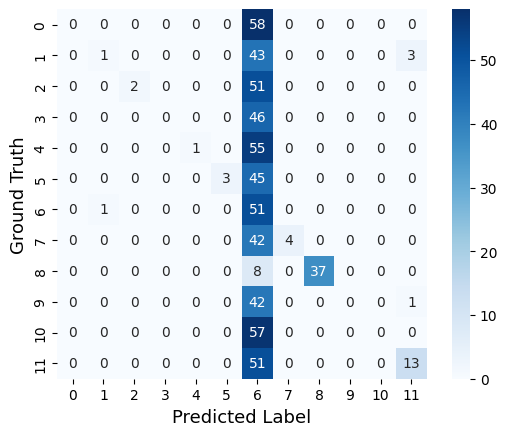
\includegraphics[width=0.6\linewidth]{./img/el.png}
\end{center}
\caption{Confusion Matrix when using ellipse fitting under close-set condition}
\end{figure}

\subsection{Applying wavelet reconstruction after applying ellipse fitting}
I got 83.41\% by applying ellipse fitting and wavelet reconstruction under close-set condition.

\begin{figure}[H]
\begin{center}
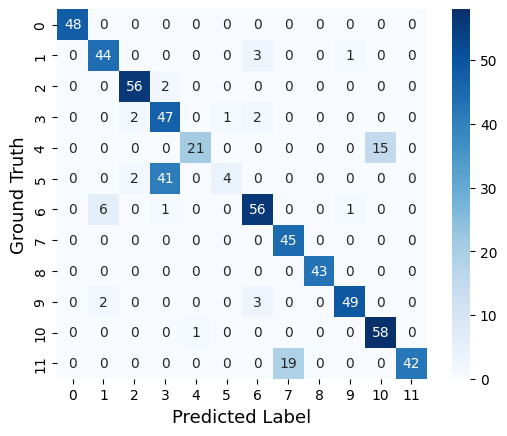
\includegraphics[width=0.6\linewidth]{./img/el_wav.png}
\end{center}
\caption{Confusion Matrix when using ellipse fitting and wavelet reconstruction under close-set condition}
\end{figure}

\section{A Result under open-set condition}
I got 44.06\% by applying same preprocessing method above under open-set condition. Six subjects' data were used in training, the other six in testing only. In fig. 2, Label 6 indicates unknown people.

\begin{figure}[H]
\begin{center}
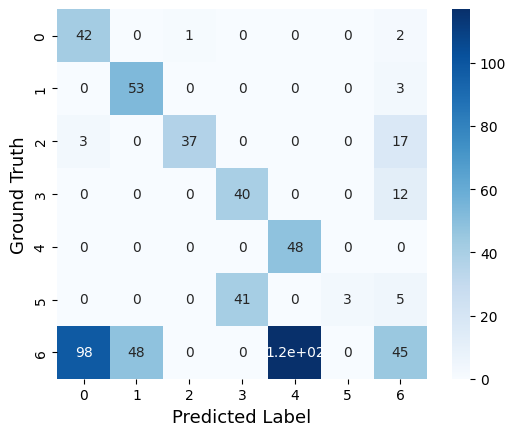
\includegraphics[width=0.6\linewidth]{./img/el_wav_open.png}
\end{center}
\caption{Confusion Matrix when using ellipse fitting and wavelet reconstruction under open-set condition}
\end{figure}

\section{Next Plan}
\begin{itemize}
    \item As you can see from the figure below, I think wavelet reconstruction has a role to remove undesired frequency band signals, I will confirm the effectiveness of wavelet reconstruction by comparing it with ellipse fitting and BPF application.
\end{itemize}

\begin{figure}[htbp]
    \begin{minipage}[c]{0.5\hsize}
      \centering
      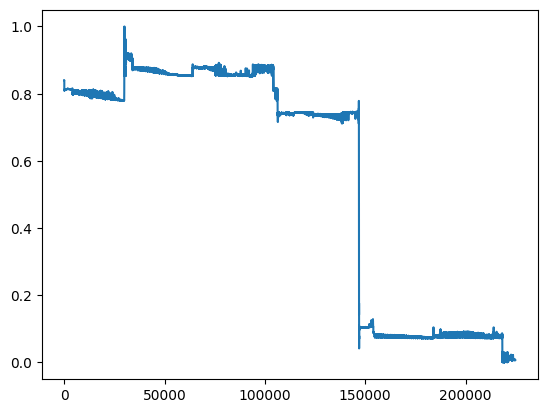
\includegraphics[width=\linewidth]{./img/wave_el.png}
      \caption{Waveform just applying ellipse fitting}
    %   \label{fig:statue}
    \end{minipage}
    \begin{minipage}[c]{0.5\hsize}
      \centering
      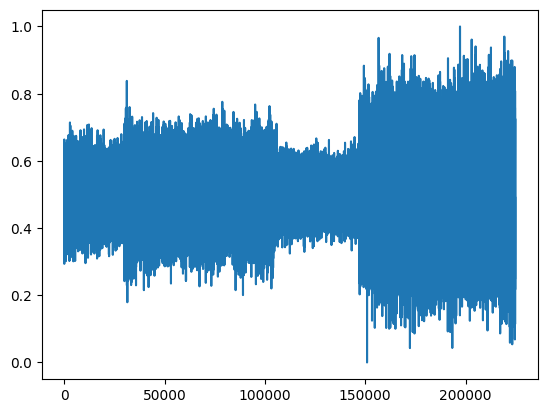
\includegraphics[width=\linewidth]{./img/wave_elwav.png}
      \caption{Waveform applying ellipse fitting and Wavelet reconstruction}
    %   \label{fig:spaceship}
    \end{minipage}
  \end{figure}

\end{document}